	En este capitulo mostramos los resultados del presente trabajo, comparamos los resultados de la ejecución de 5 modelos, los tiempos de ejecución y 
		comparamos los resultados obtenidos. Los modelos ejecutados tanto los originales, en PowerDEVS, y los modelos transformados en 
		$\mu$-Modelilca se encuentran en \url{https://github.com/lucciano/pd2mo/tree/master/doc/tesina/src}


\section{Comparación de performance}
	A continuación por cada uno de los modelos se muestra su modelo en Powerdevs seguido de una gráfica de valores en tiempo de las simulaciones, 
	a la izquierda se muestra el resultado en PowerDEVS y a la derecha los de QSS-Solver convertidos por la herramienta desarrollada.

\section{Líneas de Transmisión}
	El siguiente sistema de ecuaciones representan un modelo a parámetros concentrados de una línea de transmisión formada por $N$ secciones de circuitos LC:

\begin{equation*}
\begin{split}
\dot{v}_{j} &= \frac{i_{j} - i_{j+1}}{C} \\
\dot{i}_{j} &= \frac{v_{j-1} - v_{j}}{L} \\	
\end{split}
\end{equation*}

para $j = 1 \dots N$

Consideramos también un pulso de entrada:
\begin{equation}
v_0(t) = \left\{ 
  \begin{array}{l l}
    1 \text{ si } t < 1 \\
    0 \text{ en caso contrario }
  \end{array} \right.
\end{equation}

 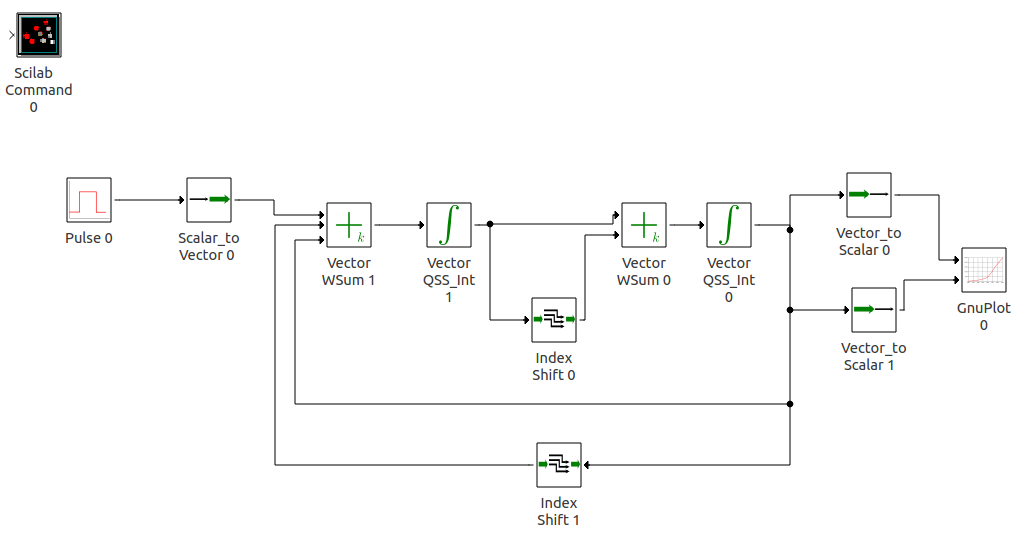
\includegraphics[width=0.75\linewidth]{lclines}

\begin{figure}[H]
\centering
\begin{minipage}{0.5\textwidth}
\centering
 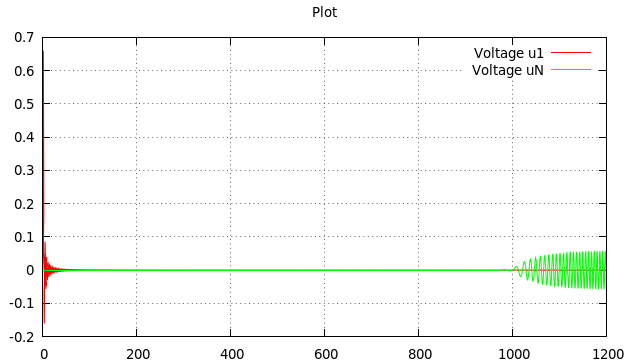
\includegraphics[width=\linewidth]{lcline-pd}
\end{minipage}\hfill
\begin{minipage}{0.5\textwidth}
\centering
 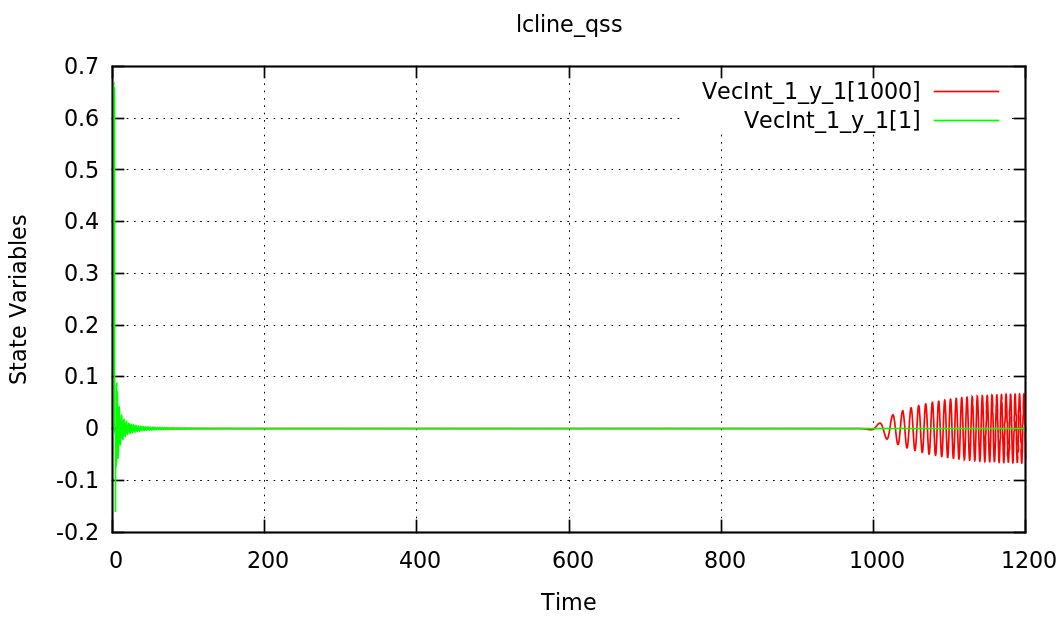
\includegraphics[width=\linewidth]{lcline-qss}
\end{minipage}
\end{figure}

\section{Inversores Lógicos}
	El siguiente modelo representa una cadena de $m$ inversores lógicos, 

\begin{align*}
\dot{\omega}_1 & = U_{op} - \omega_1(t) - \Upsilon g (u_{in}(t), \omega_{1} (t))    \\
\dot{\omega}_j & = U_{op} - \omega_j(t) - \Upsilon g (\omega_{j-1}(t), \omega_{j} (t)) \textrm{ donde $j = 2, 3, .., m$}
\end{align*}


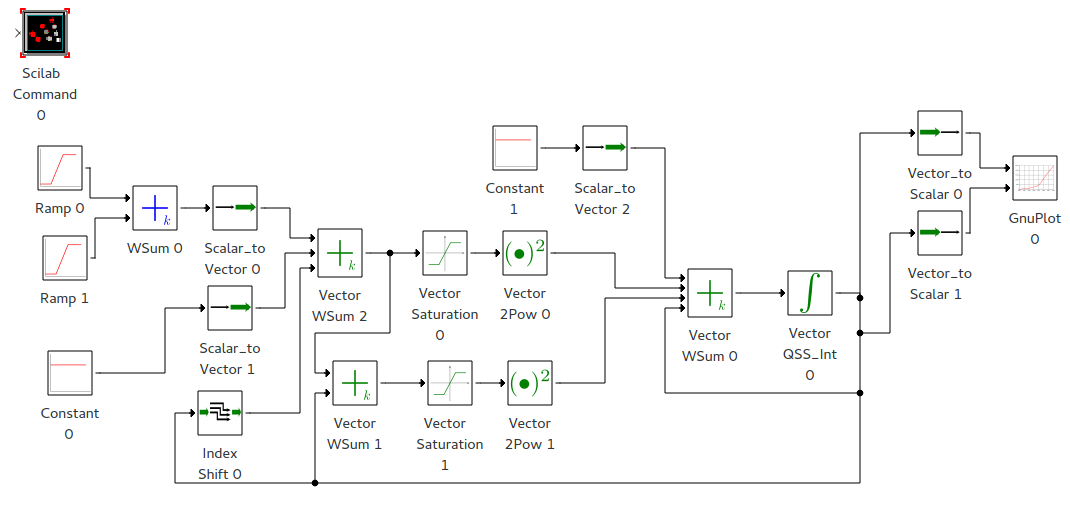
\includegraphics[width=0.75\linewidth]{inverters}

\begin{figure}[H]
\centering
\begin{minipage}{0.5\textwidth}
\centering
 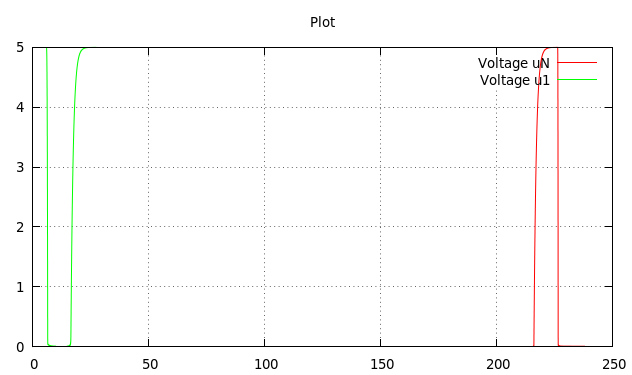
\includegraphics[width=\linewidth]{inversers-pd}
\end{minipage}\hfill
\begin{minipage}{0.5\textwidth}
\centering
 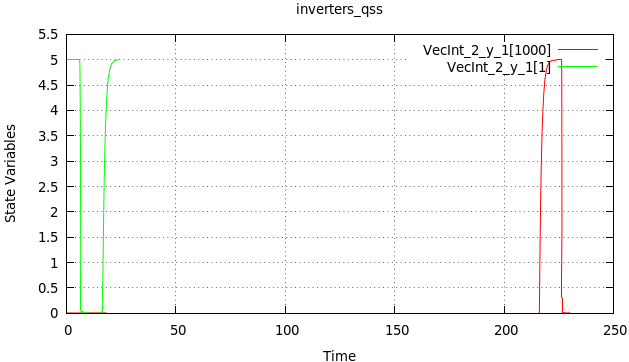
\includegraphics[width=\linewidth]{inversers-qss}
\end{minipage}
\end{figure}

\section{Advection-diffusion-reaction}
	El modelo de equaciones Advection-diffusion-reaction (ADR) provee las bases para describir fenomenos de tranferencias de calor y masa, donde la cantidad de interes $u(x,t)$ puede ser temeratura en la conducción de calor o concentración de una sustancia química.

La ecuación 
\begin{equation*}
\frac{du(x,t)}{dt} + a \frac{du(x,t)}{dx} = d\frac{d^2u(x,t}{d^2x} + r(u(x,t)^2 - u(x,t)^3)
\end{equation*}
corresponde al modelo ADR, donde $a$,$d$ y $r$ son parametros expresando coeficientes de advección, difusión y reactión

 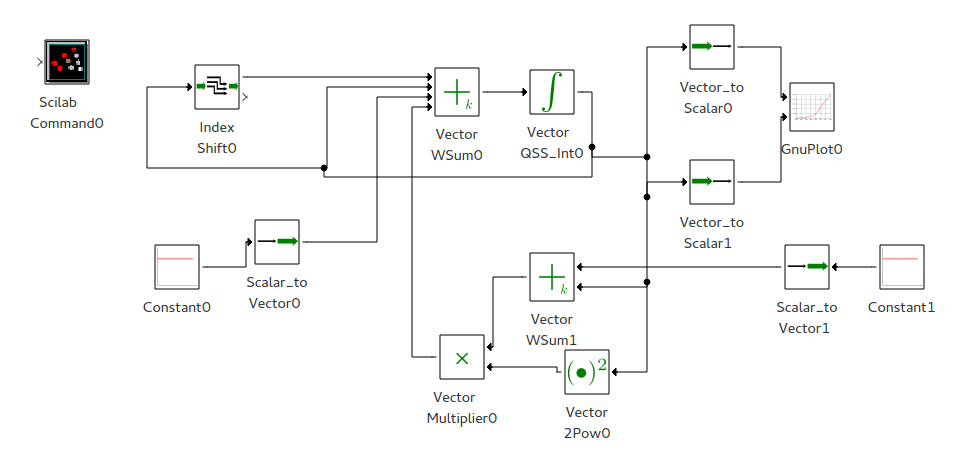
\includegraphics[width=0.75\linewidth]{adr-pwd}

\begin{figure}[H]
\centering
\begin{minipage}{0.5\textwidth}
\centering
 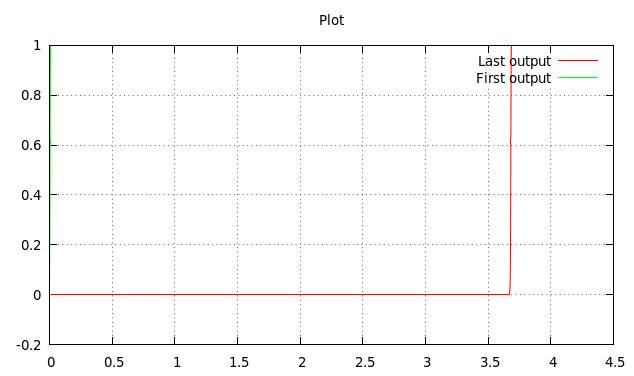
\includegraphics[width=\linewidth]{adr-pd}
\end{minipage}\hfill
\begin{minipage}{0.5\textwidth}
\centering
 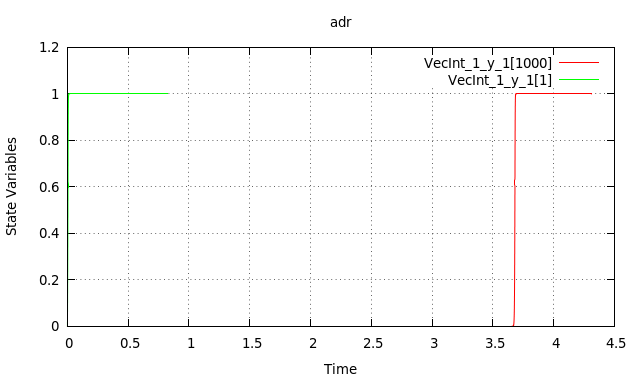
\includegraphics[width=\linewidth]{adr-qss}
\end{minipage}
\end{figure}

\section{Convertidor de Voltaje}
	El siguiente modelo es un tipo de convertidor DC - DC que obtiene a su  salida  un  voltaje  continuo  menor  que  a  su entrada, manteniendo una una  alta eficiencia (superior al 95\% con circuitos integrados) y autoregulación.

\begin{align*}
\frac{di_{L}}{dt} & = \frac{-u_{C} - R_D i_D }{L}\\
\frac{du_C}{dt} & =i_D \frac{i_D}{C} - \frac{u_C}{R_L C }
\end{align*}
donde
\begin{align*}
i_D & = \frac{R_s i_L - u_C - U }{R_D + R_s}
\end{align*}


\begin{figure}[H]
\centering
 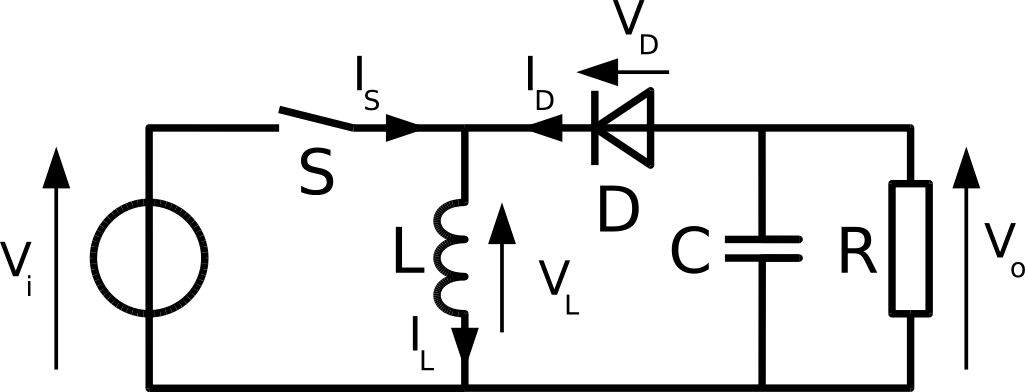
\includegraphics[width=.60\linewidth]{Buckboost_conventions}
 \caption{Esquema electrico de convertidor buck}
\end{figure}

\begin{figure}[H]
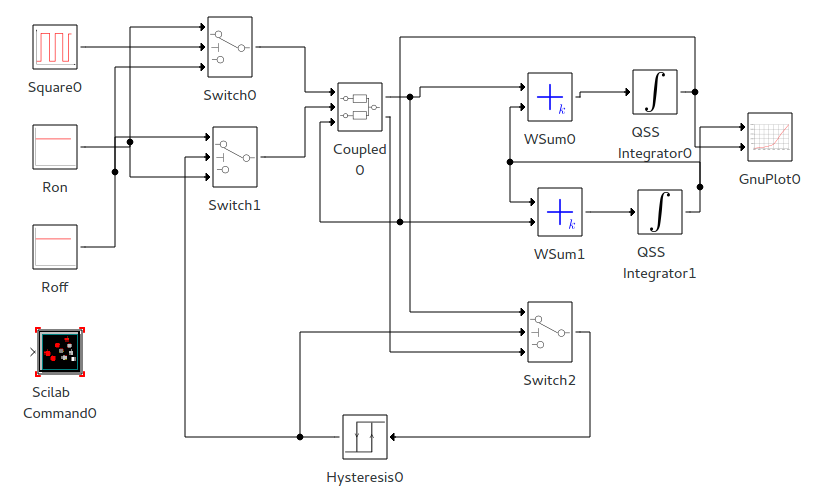
\includegraphics[width=0.75\linewidth]{buck_disk}
\caption{Modelo Buck Disk}
\end{figure}

\begin{figure}[H]
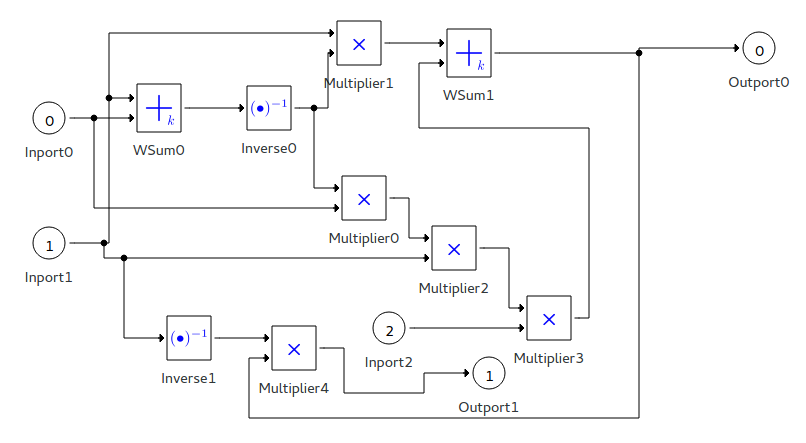
\includegraphics[width=0.75\linewidth]{buck_disk_coupled0}
\caption{Coupled0 (Incluido en Buck Disk)}
\end{figure}

\begin{figure}[H]
\centering
\begin{minipage}{0.5\textwidth}
\centering
 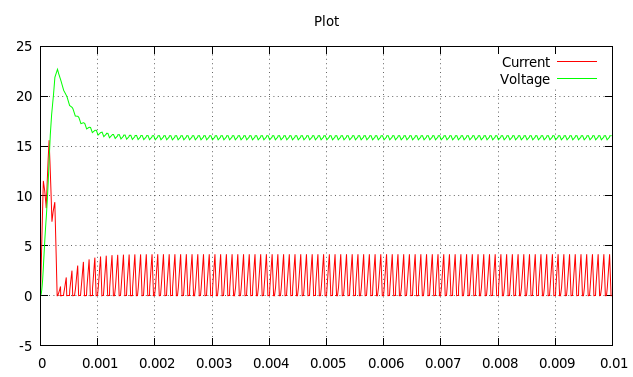
\includegraphics[width=\linewidth]{buck_disk-pd}
\end{minipage}\hfill
\begin{minipage}{0.5\textwidth}
\centering
 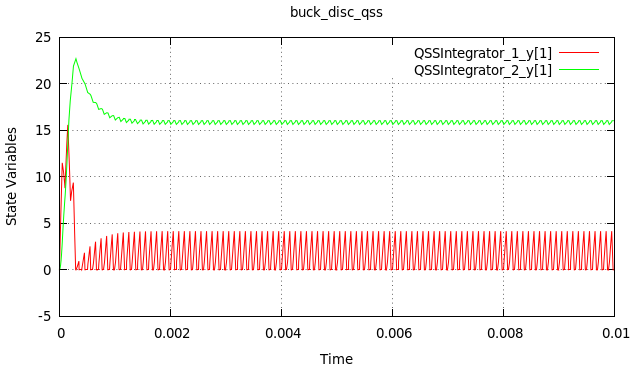
\includegraphics[width=\linewidth]{buck_disk-qss}
\end{minipage}
\end{figure}

\section{Ecuaciones Lotka-Volter}

	El sistema de ecuaciones Lotka-Volter, es un sistema de ecuaciones diferenciales de primer orden, no lineales, utilizadas para describir dinámicas de sistemas biológicos en el cual dos especies interactúan, una como presa y otra como depredador, se definen como:

\begin{align*}
\frac{dx}{dt} & = x(\alpha - \beta y)\\
\frac{dy}{dt} & =y(\gamma - \delta  x)
\end{align*}

donde:
\begin{itemize}
	\item y es el número de algún predador (por ejemplo, un lobo);
    \item x es el número de sus presas (por ejemplo, conejos);
    \item t representa el tiempo; y
    \item $\alpha$, $\beta$, $\gamma$, $\delta$ son parámetros que representan las interacciones de las dos especies.
\end{itemize}

	Este sistema es representado por el modelo siguiente:

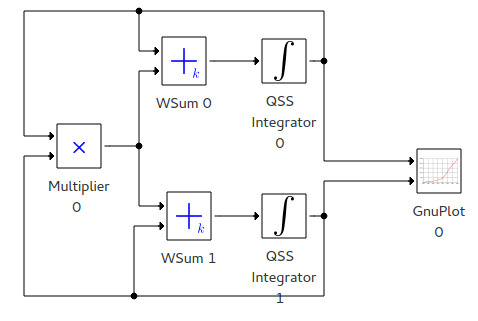
\includegraphics[width=0.75\linewidth]{lotka_voltera_pwd}

\begin{figure}[H]
\centering
\begin{minipage}{0.5\textwidth}
\centering
 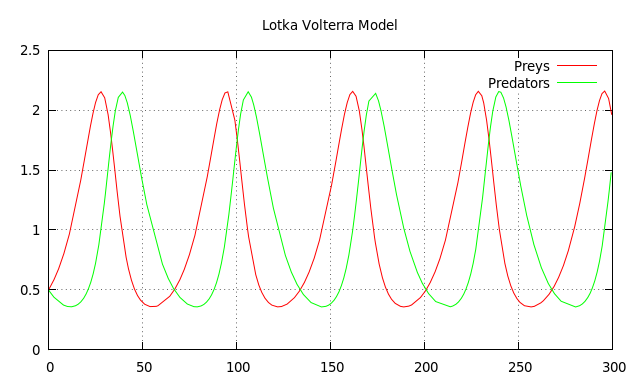
\includegraphics[width=\linewidth]{lotka_voltera-pd}
\end{minipage}\hfill
\begin{minipage}{0.5\textwidth}
\centering
 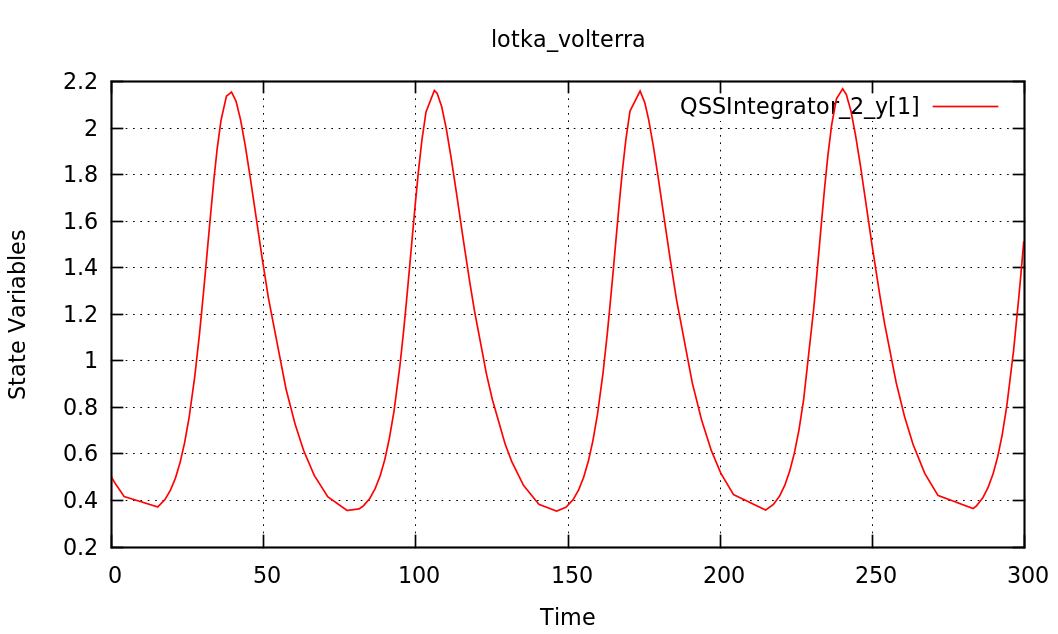
\includegraphics[width=\linewidth]{lotka_voltera-qss}
\end{minipage}
\end{figure}

\section{Resultados}

	Las pruebas fueron realizadas en una PC Intel\textsuperscript{\textregistered} Core\textsuperscript{TM} i7-3632QM CPU @ 2.20GHz con 16 GB de memoria RAM. Los tiempos observados no deben ser considerados 
	como absolutos ya que variaran de un sistema a otro, pero las mejoras relativas en los tiempos de ejecución deberían mantenerse.

	Los resultados obtenidos son los tiempos observados luego de ejecutar la simulación en PowerDEVS (P.DEVS) y QSS-Solver (QSS-S), ambas mediciones
	son reportadas por los motores de simulación, en milisegundos (ms), todas las simulaciones utilizan el método de integración QSS3 excepto los que 
	se especifica LIQSS2.

\begin{table}[H]
\centering	
\label{my-label}
\begin{tabular}{llllll}
\toprule
{\bf Modelos}            &  {\bf P.DEVS(ms)} & {\bf QSS-S. (ms)} & {\bf Mejora (\%)} \\
\toprule
Lineas de Transmisión 1200s, N=1000     & 76402         & 34982.5         & 54          \\
Inversores(LIQSS2) 250s, N=1000   	& 25046         & 7694.44         & 69        \\
ADR(LIQSS2) 10s, N=1000 		& 6089          & 568.772         & 90        \\
Convertidor de Voltaje 0.01s,        	& 268           & 10.3802         & 96         \\
Lotka  Voltera 300s      		& 11            & 2.75132         & 81

% Mejora esta calculada a partir de 1 - qsssolver / pwdevs
%excepto indicado, se utiliza QSS3
\end{tabular}
\end{table}

	En la tabla se puede ver una mejora entre 54 y 96\% entre todos los modelos, los modelos vectoriales 
